\section{Esempi di progettazione concettuale dalle slides}
\subsection{Es1 - Corso}
Cominciamo guardando un esercizio per vedere come approcciarsi allo sviluppo a partire da una specifica del tipo:
\begin{center}
    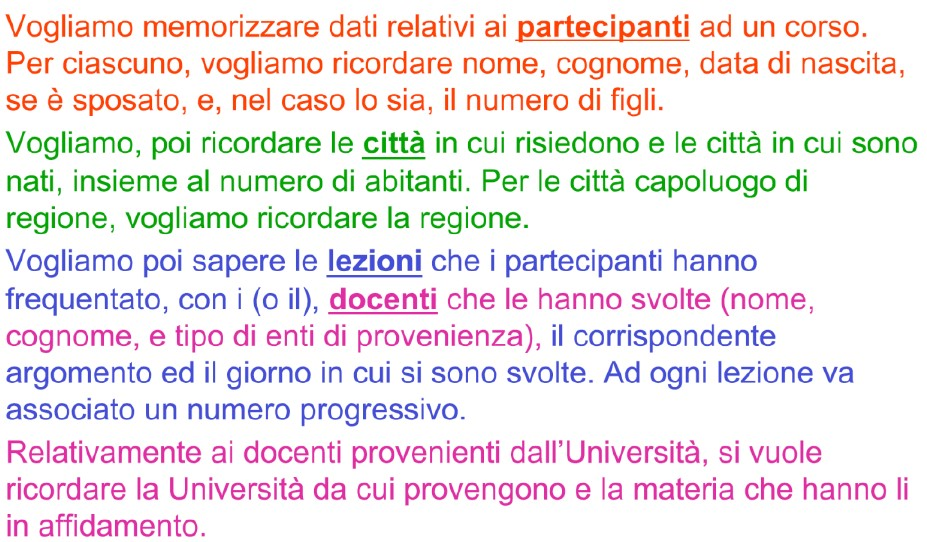
\includegraphics[width=0.675\textwidth]{chaptersLezioniSara/img/ER_es2corso_specifiche2.jpg}
\end{center}
Le specifiche sono qua colorate in modi diversi per suggerirci le parti che possono essere raggruppate in sottoinsiemi.
\\La strategia usata è quella \textbf{top-down}.
\\NB: la parte "se è sposato, e nel caso lo sia il numero dei figli", ci suggerisce che sia meglio rappresentarlo come generalizzazione piuttosto che come attributo. Stesso discorso per quanto riguarda l'entità "città" e la generalizzazione che la collega alla sotto entità "capoluogo di regione".
\begin{center}
    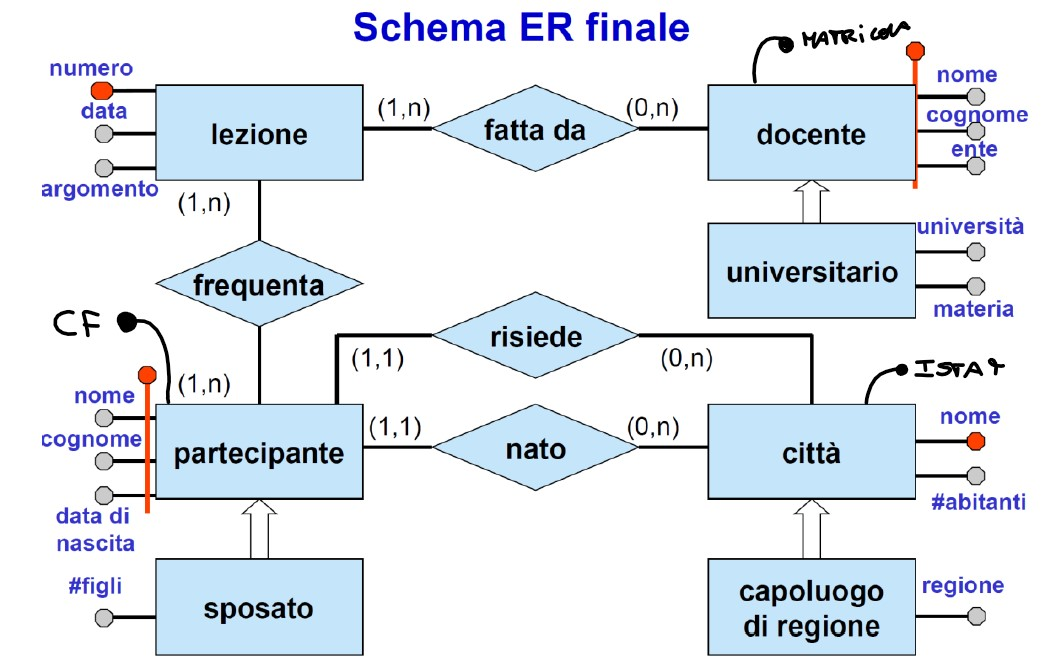
\includegraphics[width=0.675\textwidth]{chaptersLezioniSara/img/ER_es2corso_soluzioni1.jpg}
\end{center}
Qua in penna ho aggiunto varianti alla soluzione proposta che dovrebbero essere ugualmente valide.

\subsection{Es2 - Anagrafe}
\begin{center}
    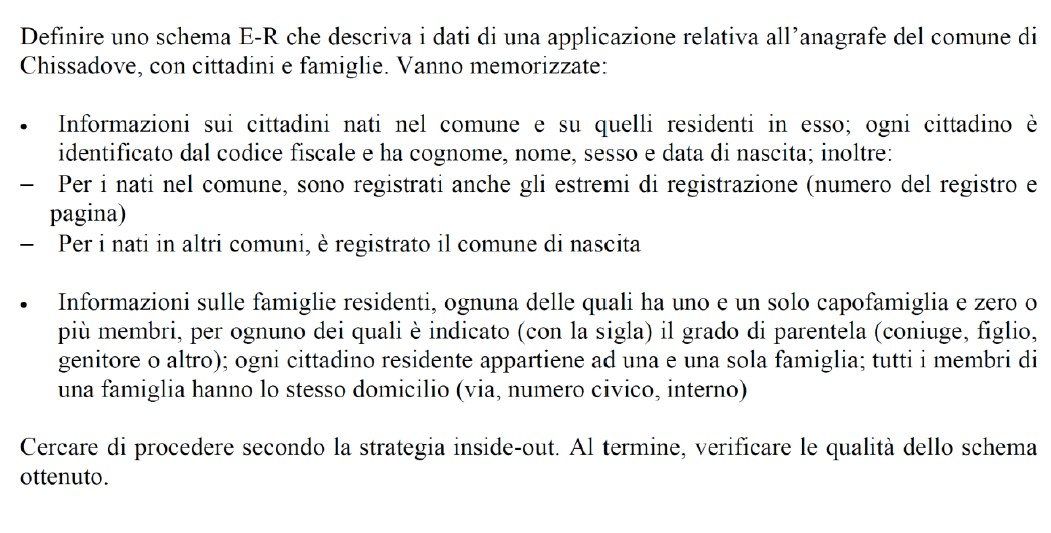
\includegraphics[width=0.675\textwidth]{chaptersLezioniSara/img/ER_es3anagrafe_specifiche1.jpg}
\end{center}
La strategia usata questa volta è quella \textbf{inside-out}.

\subsection{Es3 - Campionato}
% \begin{center}
%     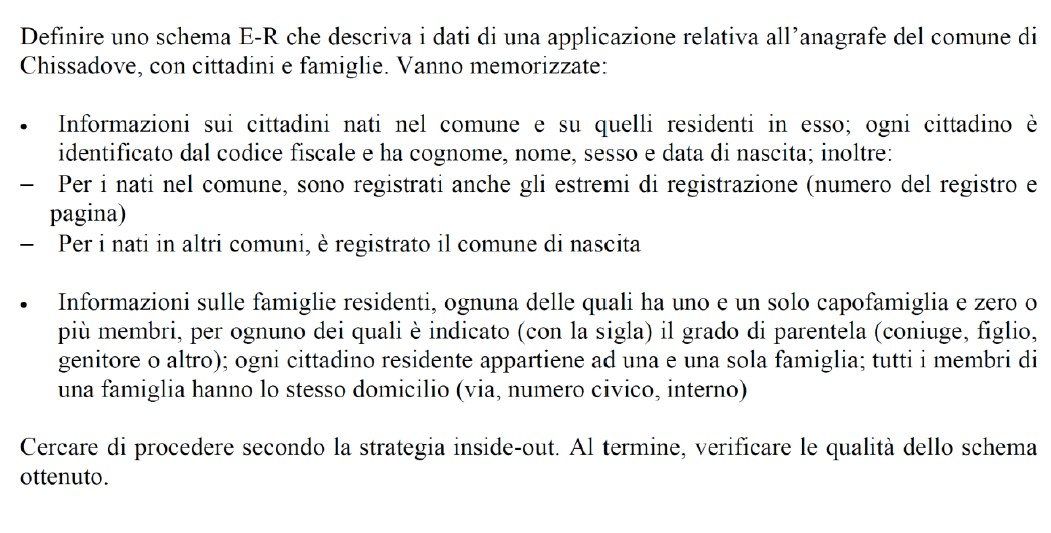
\includegraphics[width=0.675\textwidth]{chaptersLezioniSara/img/ER_es3anagrafe_specifiche1.jpg}
% \end{center}
La strategia usata questa volta è quella \textbf{top-down}.

\subsection{Es4 - Società di formazione}
Riprendiamo quanto visto a inizio lezione.
% \begin{center}
%     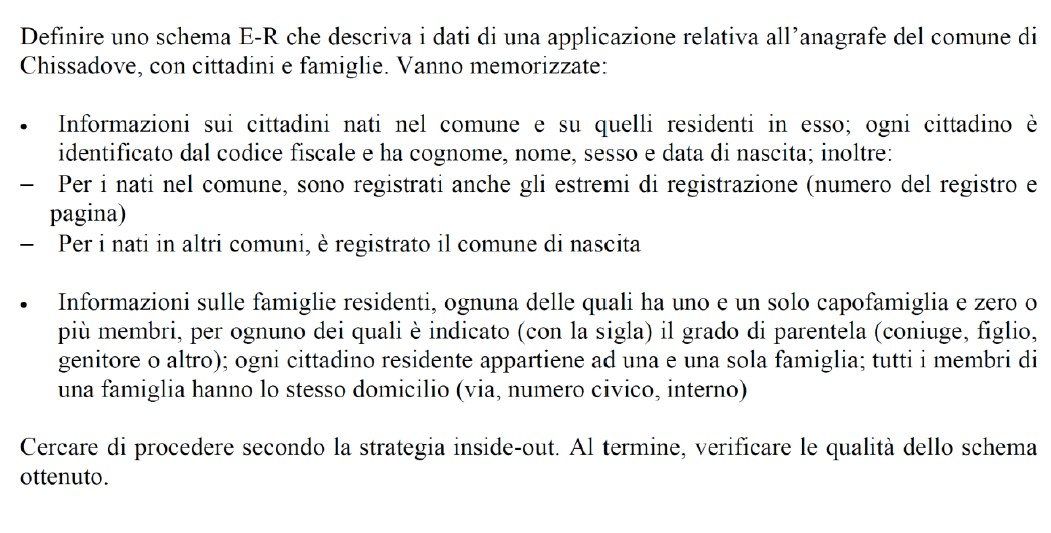
\includegraphics[width=0.675\textwidth]{chaptersLezioniSara/img/ER_es3anagrafe_specifiche1.jpg}
% \end{center}
La strategia usata questa volta è quella \textbf{top-down}.